\subsection{Background}
\subsubsection{Image processing}
An image can be seen as a mathematical function $i(x,y)$ where $x$ and $y$ are the spatial coordinates and the output is a color at position $(x,y)$. If the color has discrete quantities and the total image has a finite amount of samples, it is called a \emph{Digital Image}\cite{ipbook}. The samples each has a unique spatial coordinate and are referred to as \emph{pixels}. The field of \emph{Digital Image Processing} refers to processing a digital image and its pixels. Every time Image Processing is mentioned in this thesis, it is assumed that it refers to Digital Image Processing. 
\newline

The most typical application in image processing is when an algorithm is used on an input image to create a modified output image. Operations such as blur, sharpen and noise removal are all examples of this and are commonly used in standard image editing software. Figure \ref{lena} shows an example of a blur operation.
\begin{figure}[ht!]
\centering
\includegraphics[width=80mm]{img/klas.png}
\caption{A blur algorithm is applied on an input image and produces a blurred output image.}
\label{lena}
\end{figure}

Another possible application is when a function is used to extract information and features in an image. Figure \ref{feature} shows an example of a feature detection algorithm performed on an image of a face. The algorithm manages to locate features such as the nose, the mouth and the eyes. Although the image is processed, not everyone agrees that this is the typical application of image processing. Some people think these kind of problems belong to the computer vision field. 

\begin{figure}[ht!]
\centering
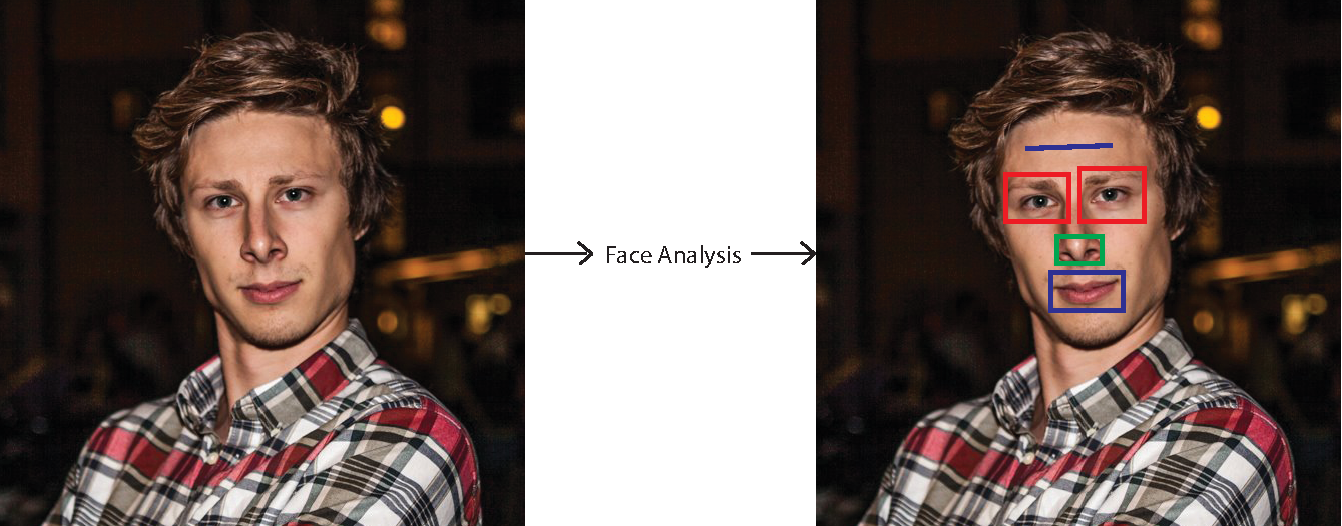
\includegraphics[width=80mm]{img/feature.pdf}
\caption{The input is analyzed to find features such as the nose, the mouth and the eyes.}
\label{feature}
\end{figure}

\subsubsection{The evolution of computing hardware}

In the early 1960s, computers finally had enough computing power to perform meaningful image processing. The \emph{Jet Propulsion Laboratory} processed images of the moon where they corrected image distortion caused by the on-board camera on the space probe \emph{Ranger 7}\cite{ipbook}. Later on, fields such as medical imaging and astronomy started to explore the field of image processing. 
\newline

As the years passed by, the capacity of the computing hardware found in computers would keep improving. The term \emph{Moore's Law}\cite{mooreslaw} was introduced based on a statement from the co-founder of Intel Corporation saying that the transistor count in integrated circuits would be increasing by a factor of two every year. In the early 1980s, a \emph{Central Processing Unit}, CPU, ran with internal clocks operating around 1 MHz. Today, around 30 years later, most CPUs have clock speeds around 2-4 GHz, which are three magnitudes faster. The faster a processor's clock is operated, the faster a floating point computation can be performed. Figure \ref{intelcpu} gives an overview of the transistor count and clock speeds of Intel CPUS\cite{mooreslawdata}.
\newline
\begin{figure}[ht!]
\centering
\includegraphics[width=110mm]{img/cpu.png}
\caption{The CPU transistor count has been growing exponentionally.}
\label{intelcpu}
\end{figure}

Due to power and heat restrictions and the physical size of the current transistors, it is hard to keep improving the clock speeds. The focus has recently shifted towards parallel computing and multicore processing units.

\subsubsection{GPU computing}

Computer games started became more popular in the 1990s. Computing was the big bottleneck in 3D graphics and it was hard to produce good real-time solutions. Therefore, companies started to experiment with a new computing device, the \emph{Graphical Processor Unit}, GPU. Instead of doing everything on the CPU, lighting computations and transformation of 3D coordinates could now be done entirely on the GPU. Since the computations of each pixels could be calculated independently of the others, it motivated the use of parallelism. 

\begin{figure}[ht!]
\centering
\includegraphics[width=90mm]{img/flops.png}
\caption{A comparison of theoretical floating point operations per second between CPUs and GPUs. This graph is from the CUDA Programming Guide\cite{cudapguide}.}
\label{flops}
\end{figure}

When a GPU uses its full power and all computing units are used to maximum efficiency, a GPU is a lot faster than a CPU in terms of floating point operations per second. Figure \ref{flops} shows a comparison between the most recent CPUs and GPUs. The reason why the GPU has lot higher theoretical maximum is because it is specalized for compute-intensive and highly parallel computations. It is therefore designed in a way where more transistors are devoted for data processing rather than data caching and flow control (which a CPU handles a lot better)\cite{cudaexample}. 
